\documentclass[11pt]{article}

\usepackage[letterpaper,margin=0.75in]{geometry}
\usepackage{booktabs}
\usepackage{caption}
\usepackage{graphicx}
\usepackage{listings}
\usepackage{float}
\usepackage{scrextend}
\usepackage{hyperref}
\usepackage[parfill]{parskip}
\renewcommand{\lstlistingname}{Snippet}


\begin{document}

\lstset{
  language=Python,
  basicstyle=\small,          % print whole listing small
  keywordstyle=\bfseries,
  identifierstyle=,           % nothing happens
  commentstyle=,              % white comments
  stringstyle=\ttfamily,      % typewriter type for strings
  showstringspaces=false,     % no special string spaces
  numbers=left,
  numberstyle=\tiny,
  numbersep=5pt,
  frame=tb
}

\title{Congestion Control Part 2}

\author{Brandt Elison & Joe Eklund}

\date{March 29, 2016}

\maketitle

\section{Introduction}

Bacon ipsum dolor amet ham hock beef pancetta, kielbasa pork belly picanha sirloin fatback shoulder. Porchetta short ribs tenderloin, filet mignon beef boudin pastrami landjaeger. Ball tip drumstick shankle pancetta porchetta brisket pork chop beef ribs flank leberkas doner ground round sausage corned beef landjaeger. Shank cupim meatball brisket.

Pork ball tip pastrami tongue pig. Tenderloin pork chop t-bone spare ribs turducken. Bacon chuck fatback turkey sausage bresaola, leberkas ham kielbasa tenderloin chicken shankle ribeye. Venison strip steak tenderloin doner porchetta. Pork belly alcatra shoulder strip steak capicola ham hock tenderloin turkey swine boudin meatloaf corned beef ham cow. Ground round venison swine bacon ham hock tongue capicola pork loin picanha frankfurter.

\section{Basic Experiments}


\begin{enumerate}
  \item One Flow
  
\begin{figure}[H]
\caption{The graph of our one flow receiver's rate over time.}
	\label{figure1}
  	\centering
  	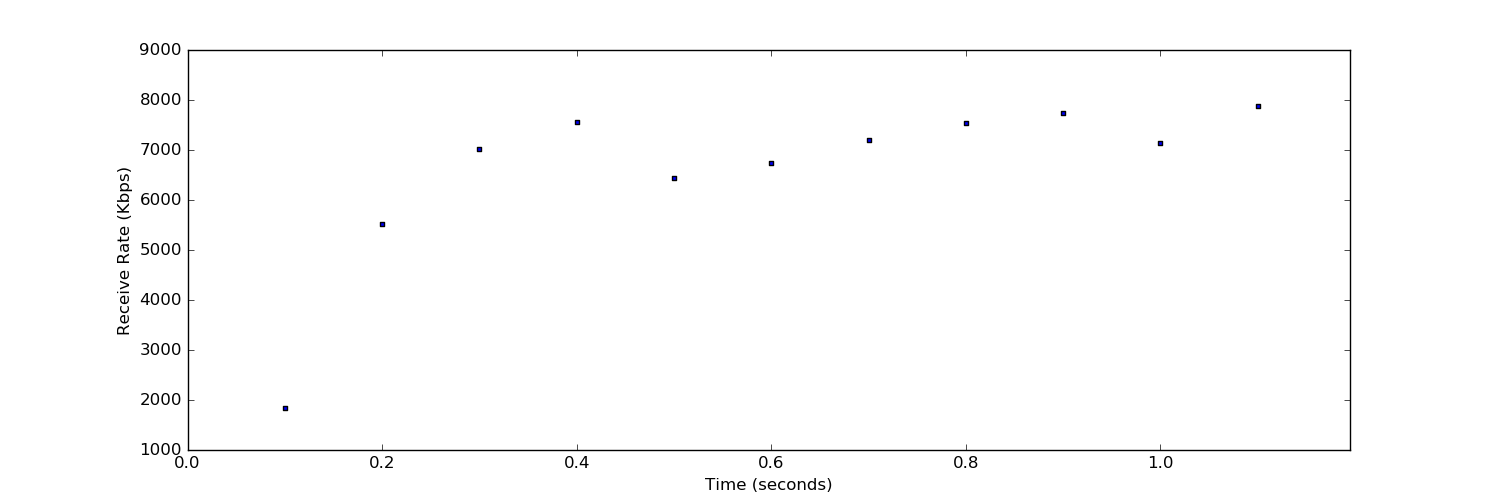
\includegraphics[width=\linewidth]{1f_rate.png}
\end{figure}

\begin{figure}[H]
\caption{The graph of our one flow queue size over time.}
  \label{figure2}
    \centering
    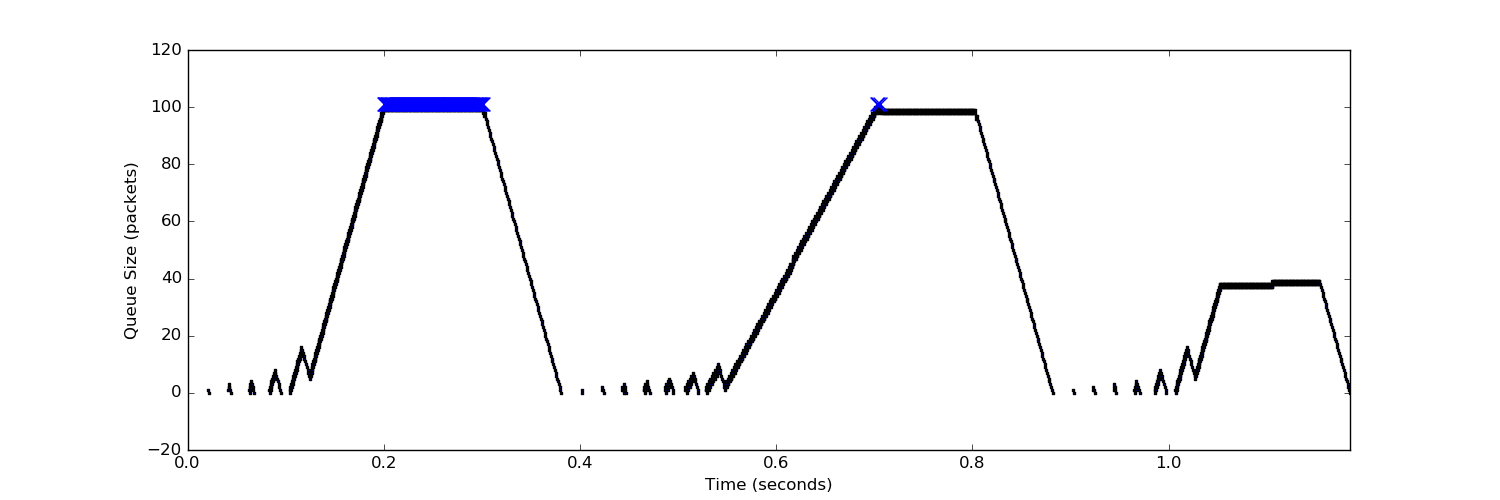
\includegraphics[width=\linewidth]{1f_queue.png}
\end{figure}

\begin{figure}[H]
\caption{The graph of our one flow congestion window size over time.}
  \label{figure3}
    \centering
    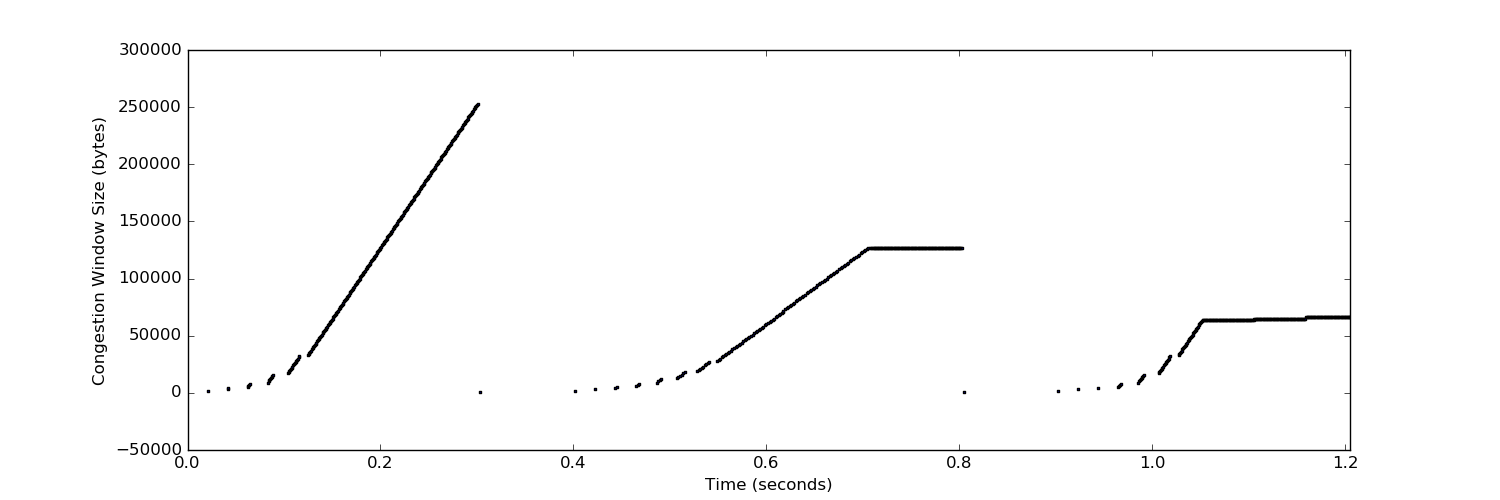
\includegraphics[width=\linewidth]{1f_window.png}
\end{figure}

\begin{figure}[H]
\caption{The graph of our one flow sequence plot.}
  \label{figure4}
    \centering
    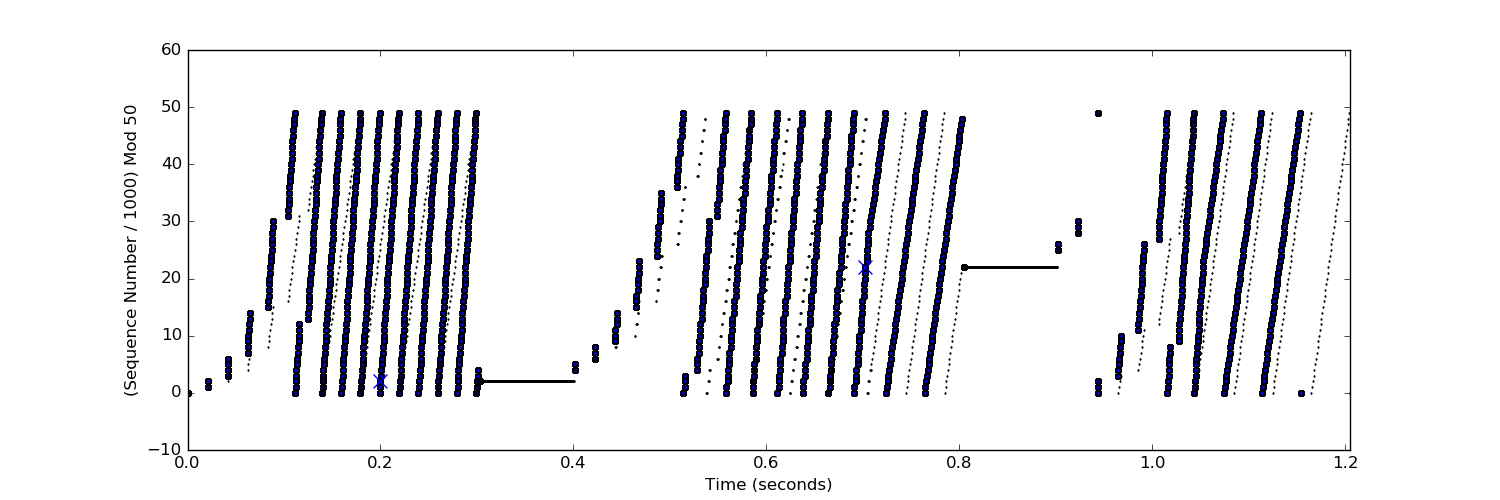
\includegraphics[width=\linewidth]{1f_seq.png}
\end{figure}

discuss one flow here

\bigskip
\item Two Flow

\begin{figure}[H]
\caption{The graph of our two flow receivers' rates over time.}
  \label{figure5}
    \centering
    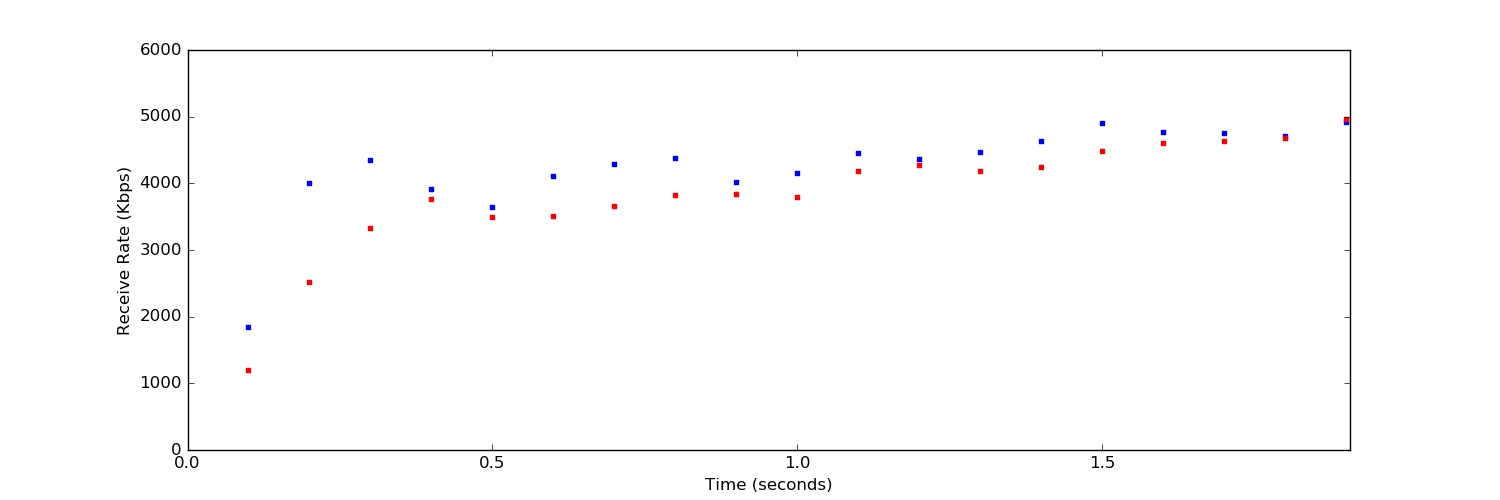
\includegraphics[width=\linewidth]{2f_rate.png}
\end{figure}

\begin{figure}[H]
\caption{The graph of our two flow queue size over time.}
  \label{figure6}
    \centering
    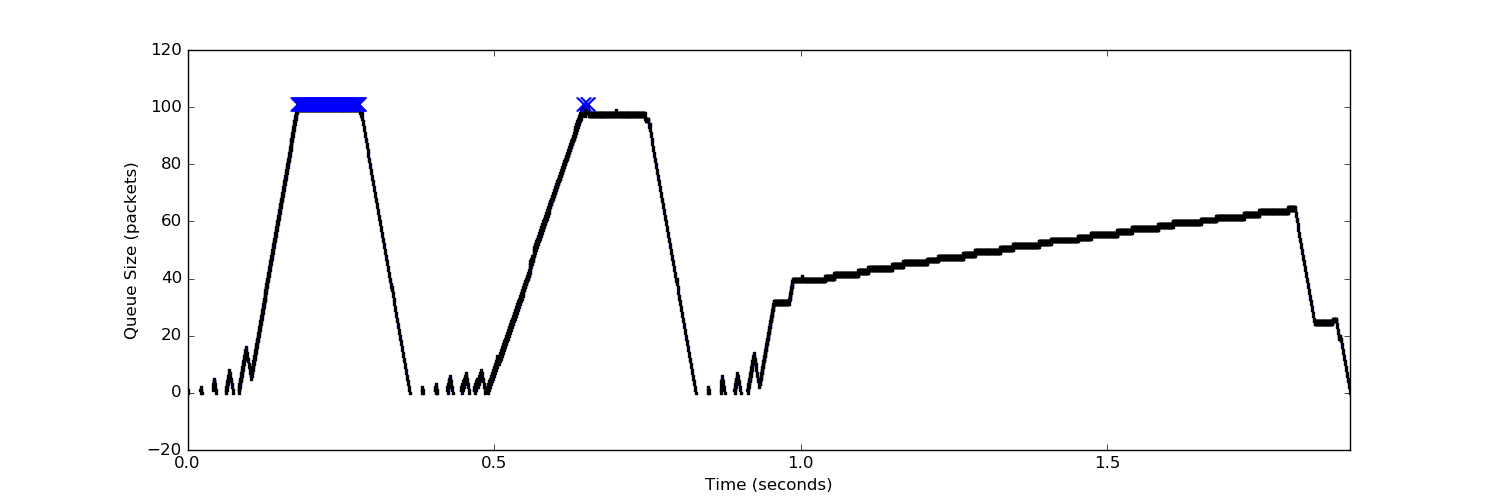
\includegraphics[width=\linewidth]{2f_queue.png}
\end{figure}

\begin{figure}[H]
\caption{The graph of our two flow congestion window size over time for flow A.}
  \label{figure7}
    \centering
    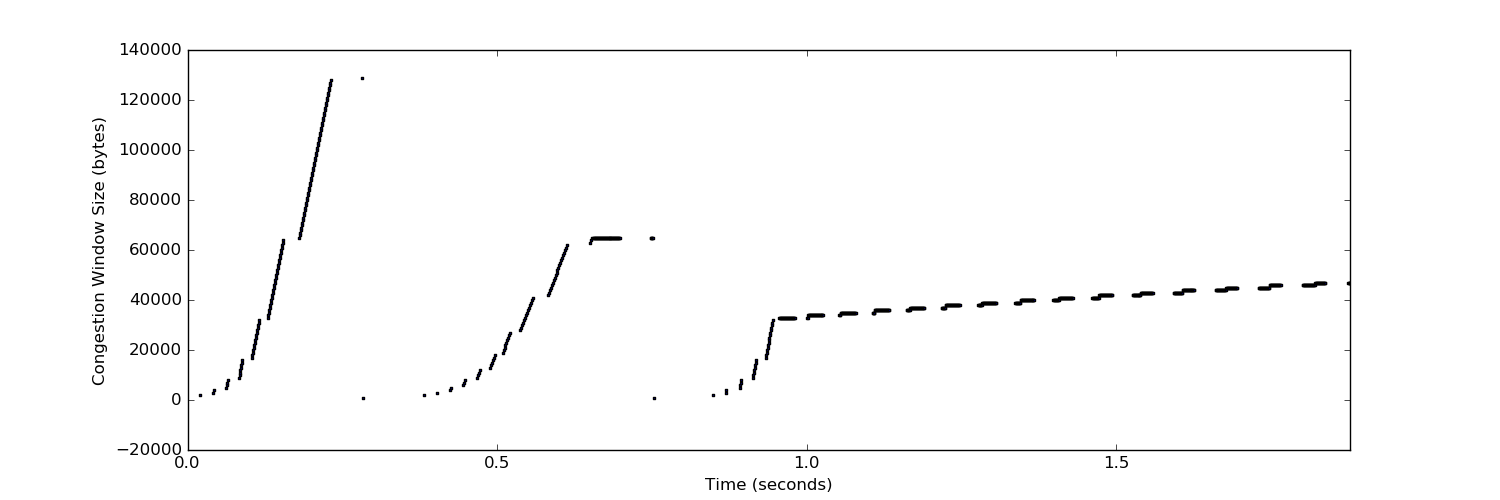
\includegraphics[width=\linewidth]{2f1_window.png}
\end{figure}

\begin{figure}[H]
\caption{The graph of our two flow congestion window size over time for flow B.}
  \label{figure8}
    \centering
    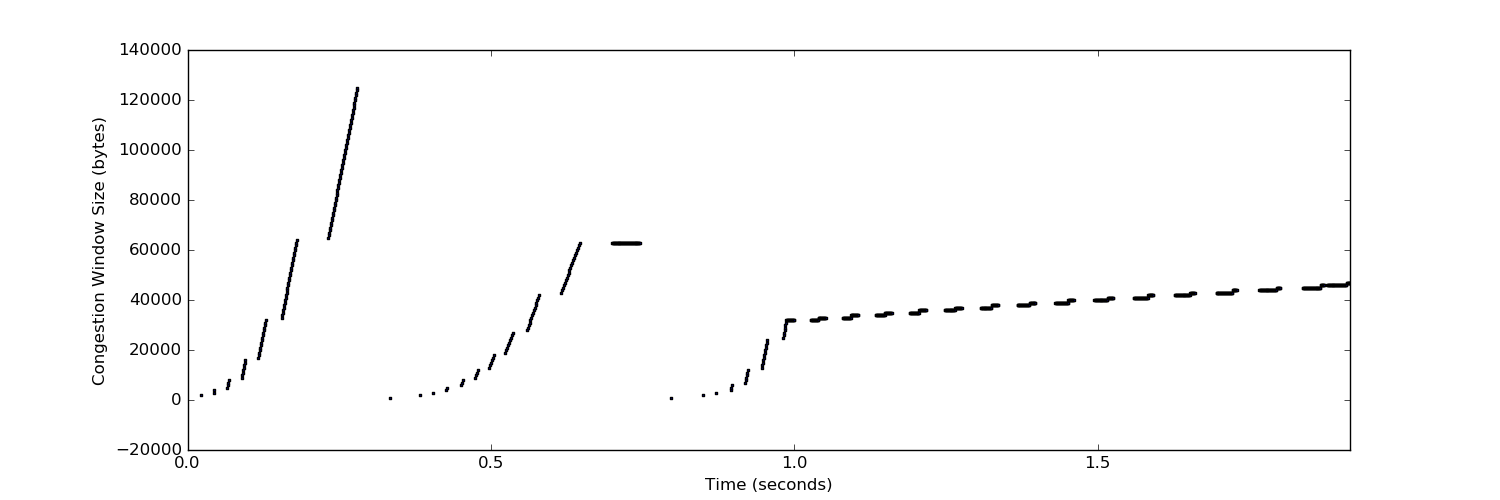
\includegraphics[width=\linewidth]{2f2_window.png}
\end{figure}

\begin{figure}[H]
\caption{The graph of our two flow sequence plot for flow A.}
  \label{figure9}
    \centering
    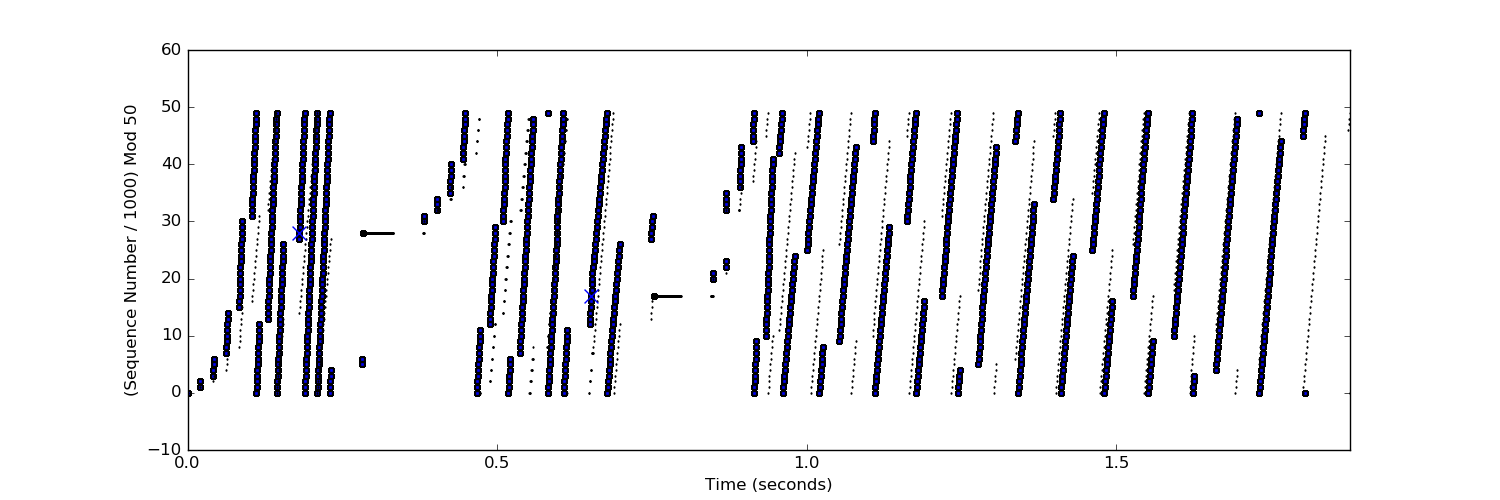
\includegraphics[width=\linewidth]{2f1_seq.png}
\end{figure}

\begin{figure}[H]
\caption{The graph of our two flow sequence plot for flow B.}
  \label{figure10}
    \centering
    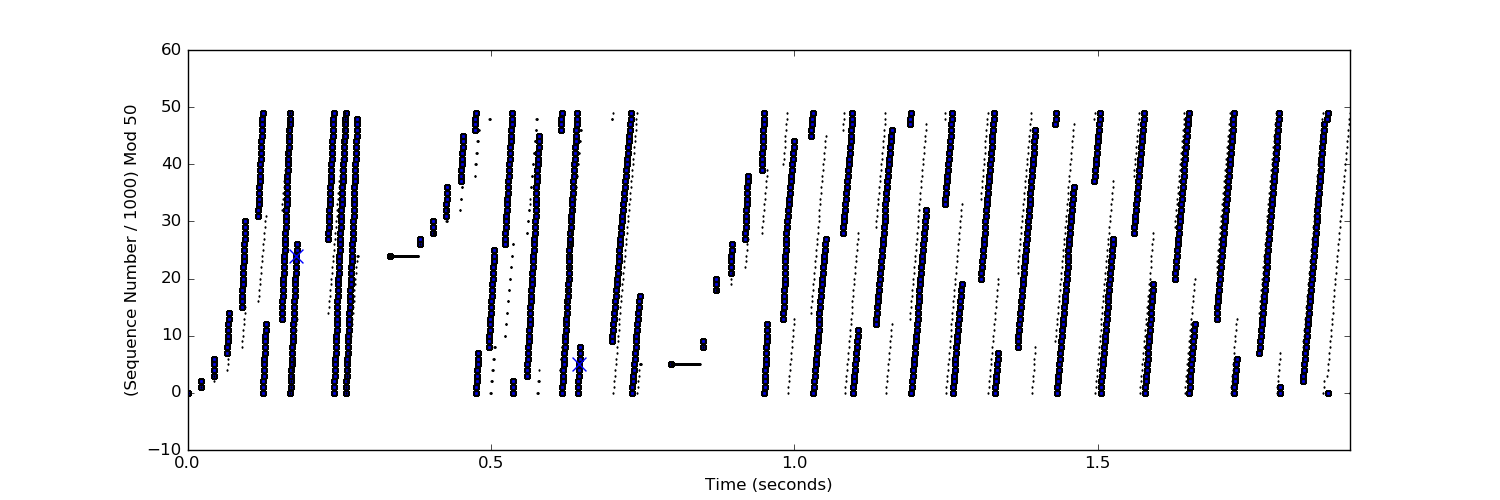
\includegraphics[width=\linewidth]{2f2_seq.png}
\end{figure}

discuss two flow here

\bigskip
  \item Five Flow

\begin{figure}[H]
\caption{The graph of our five flow receivers' rates over time.}
  \label{figure11}
    \centering
    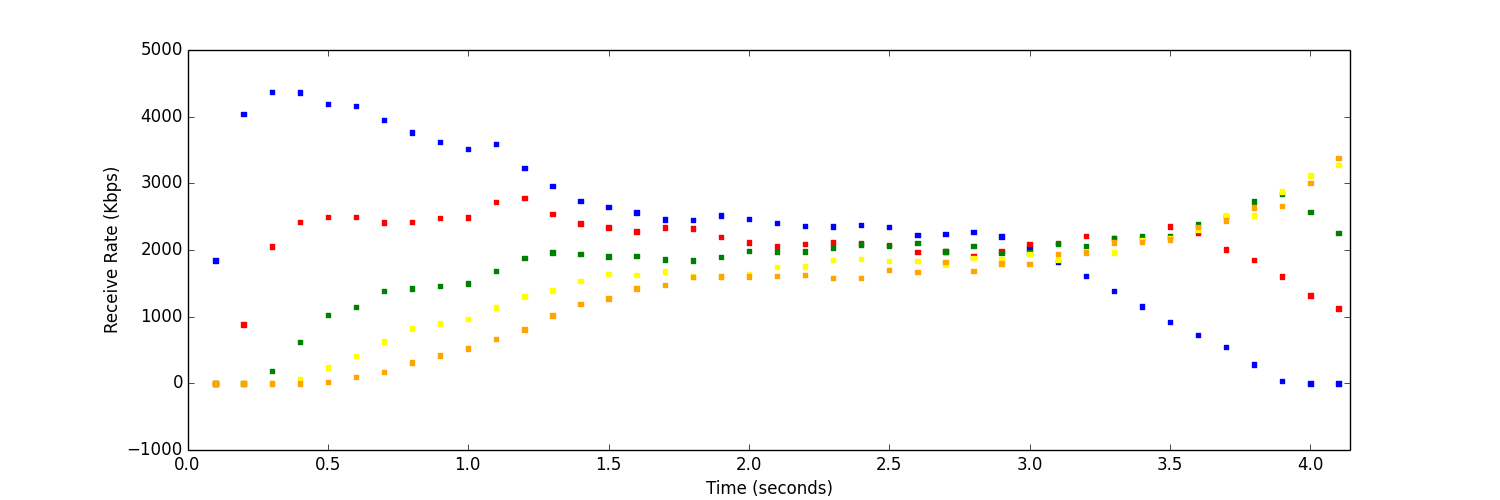
\includegraphics[width=\linewidth]{5f_rate.png}
\end{figure}

\begin{figure}[H]
\caption{The graph of our five flow queue size over time.}
  \label{figure12}
    \centering
    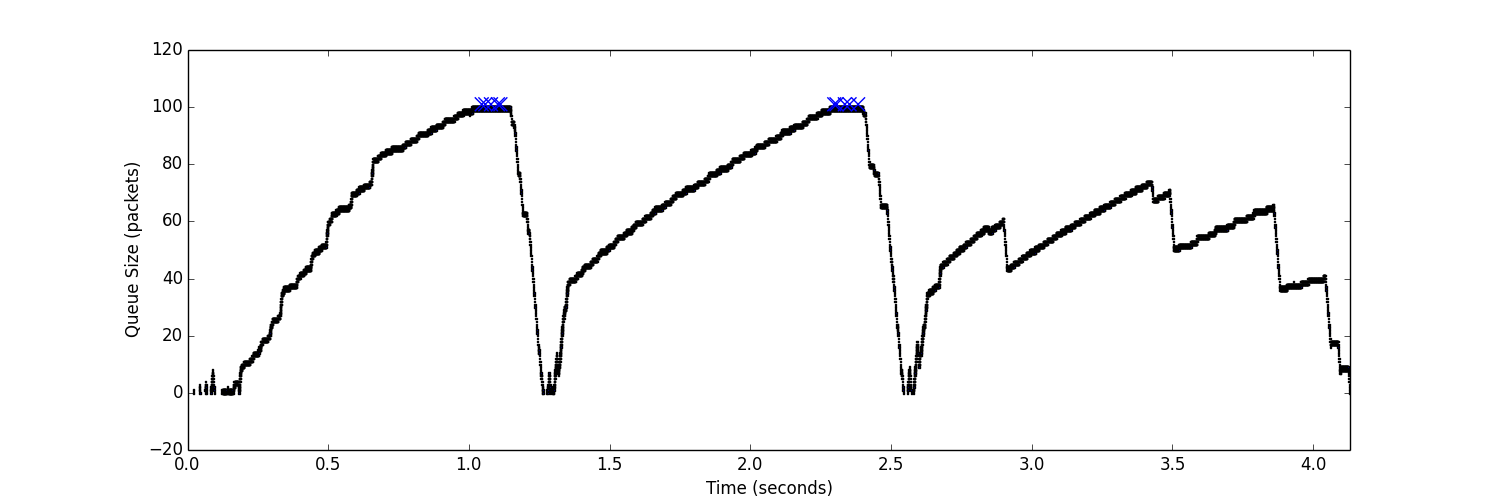
\includegraphics[width=\linewidth]{5f_queue.png}
\end{figure}

discuss five flow here

\end{enumerate}

\section{Advanced Experiments}

\begin{enumerate}
\item AIAD

\begin{figure}[H]
\caption{The graph of our one flow receiver's rate over time with AIAD.}
  \label{figure13}
    \centering
    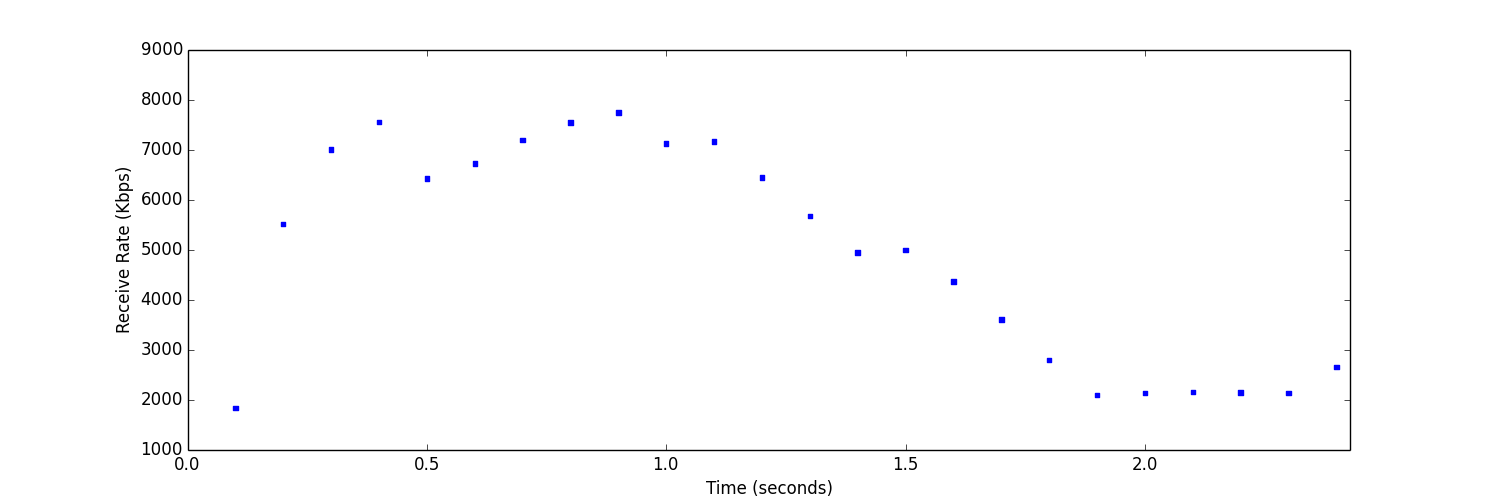
\includegraphics[width=\linewidth]{1f_rateAIAD.png}
\end{figure}

\begin{figure}[H]
\caption{The graph of our one flow congestion window size over time with AIAD.}
  \label{figure14}
    \centering
    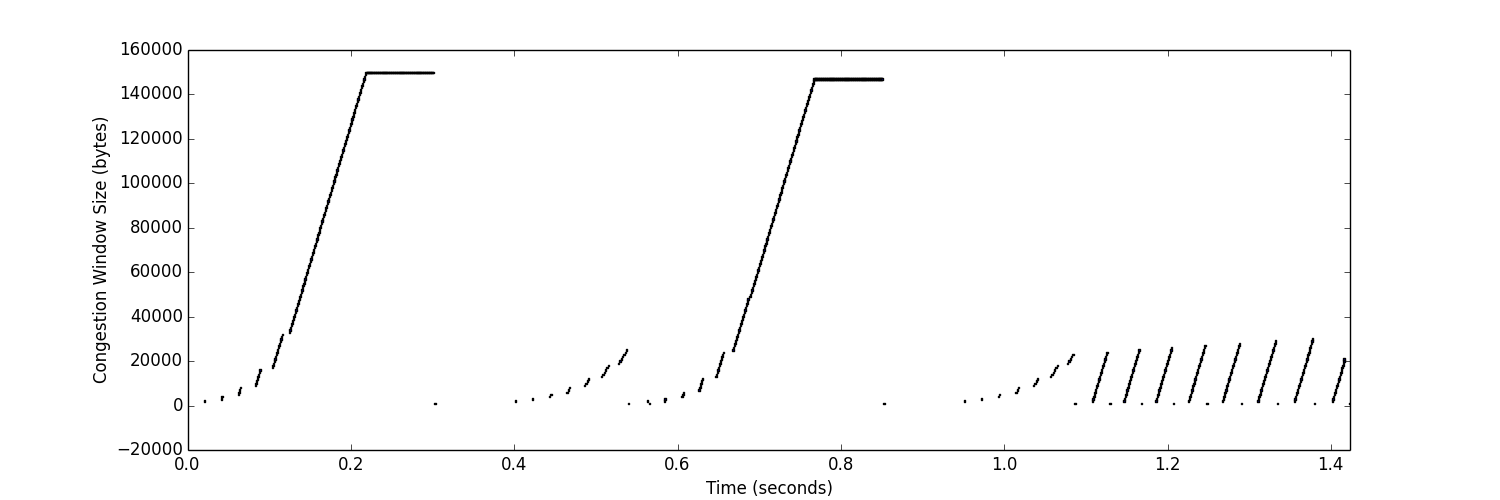
\includegraphics[width=\linewidth]{1f_windowAIAD.png}
\end{figure}


discuss AIAD here

\bigskip
\item AIMD

\begin{figure}[H]
\caption{The graph of our one flow receiver's rate over time with a 5/6 multiplicative decrease.}
  \label{figure15}
    \centering
    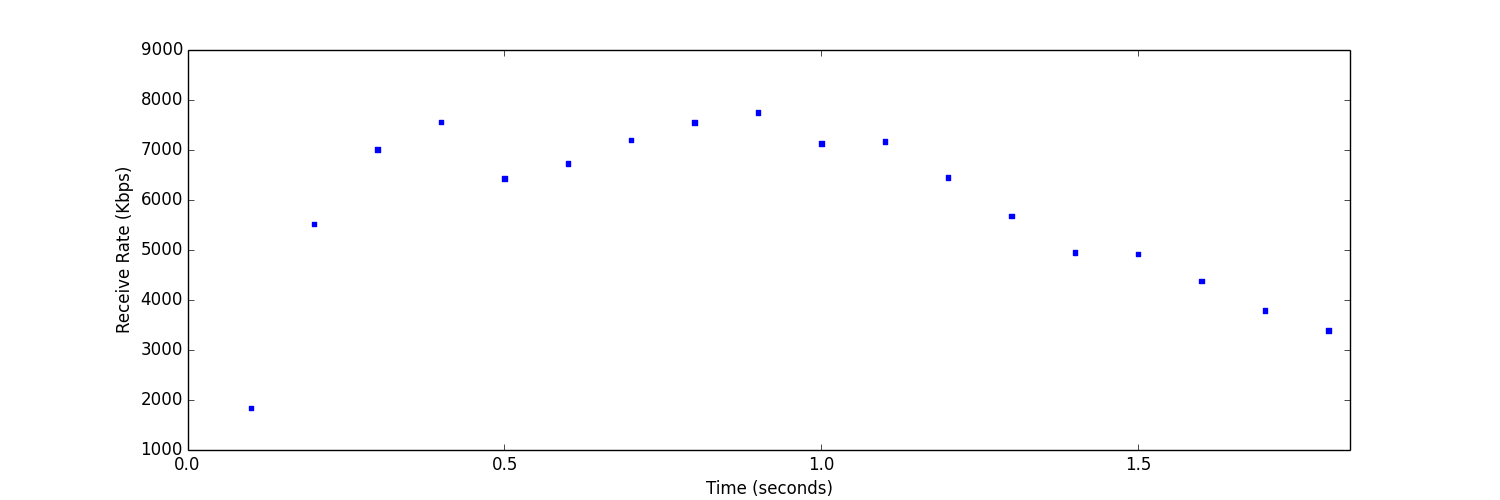
\includegraphics[width=\linewidth]{1f_rateAIMD.png}
\end{figure}

\begin{figure}[H]
\caption{The graph of our one flow congestion window size over time with a 5/6 multiplicative decrease.}
  \label{figure16}
    \centering
    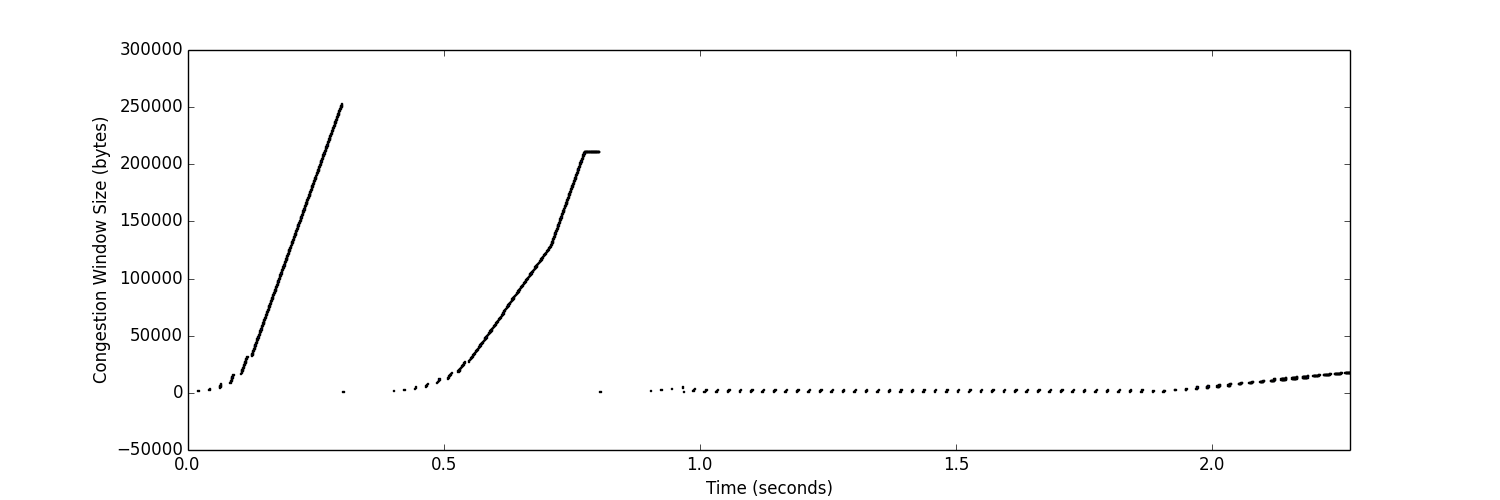
\includegraphics[width=\linewidth]{1f_windowAIMD.png}
\end{figure}

discuss AIMD here

\bigskip
\item Competing AIMD

\begin{figure}[H]
\caption{The graph of our two flow receivers' rates over time with competing AIMD.}
  \label{figure15}
    \centering
    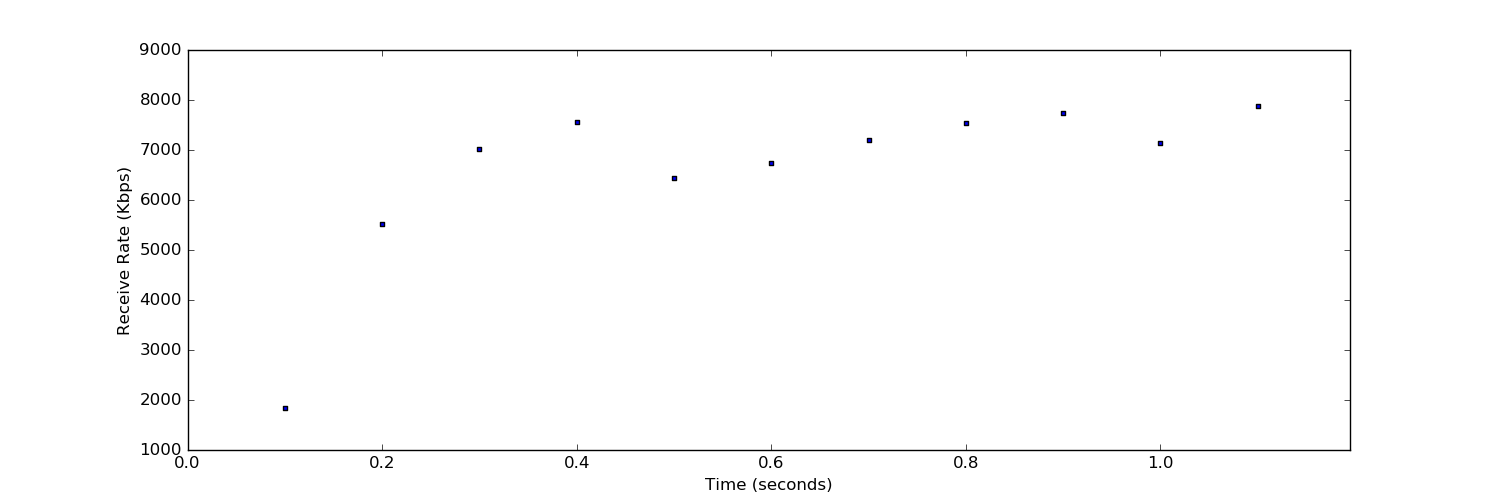
\includegraphics[width=\linewidth]{1f_rate.png}
\end{figure}

\begin{figure}[H]
\caption{The graph of our two flow congestion window size over time with competing AIMD.}
  \label{figure16}
    \centering
    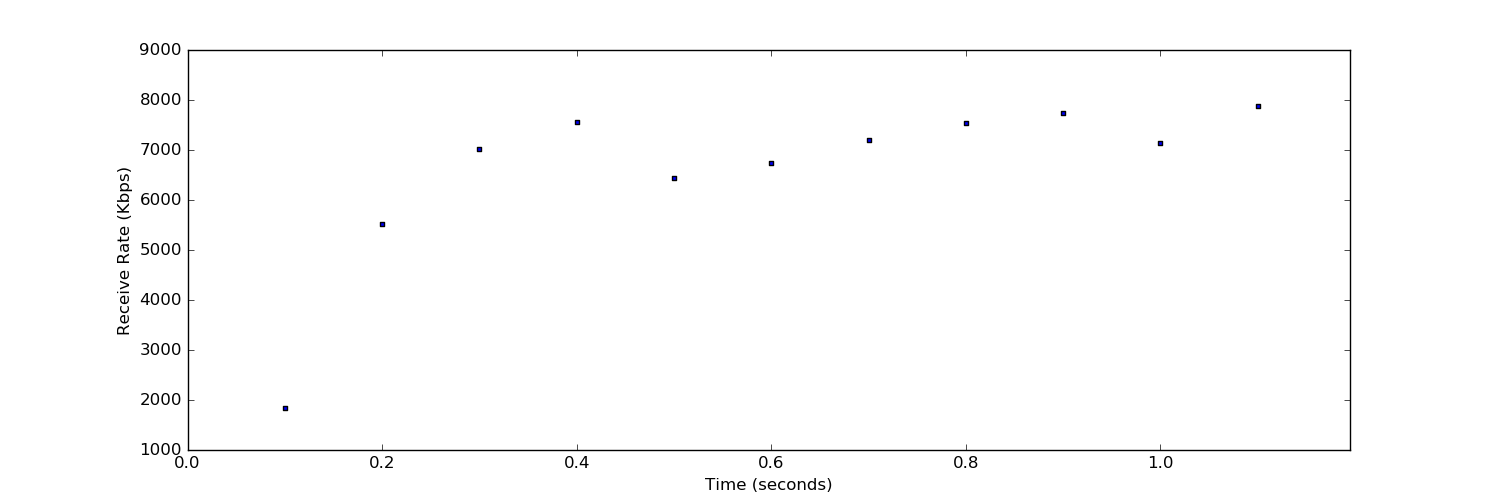
\includegraphics[width=\linewidth]{1f_rate.png}
\end{figure}

discuss competing AIMD here

\bigskip
\item Competing RTT

\begin{figure}[H]
\caption{The graph of our two flow receivers' rates over time with competing RTT.}
  \label{figure17}
    \centering
    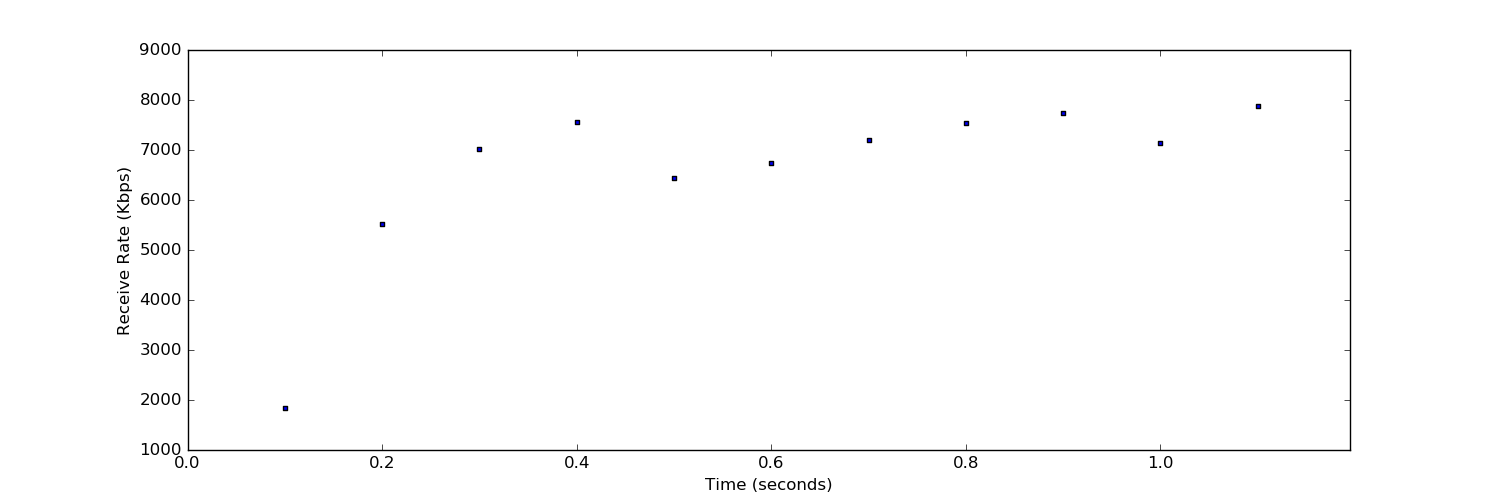
\includegraphics[width=\linewidth]{1f_rate.png}
\end{figure}

\begin{figure}[H]
\caption{The graph of our two flow congestion window size over time with competing RTT.}
  \label{figure18}
    \centering
    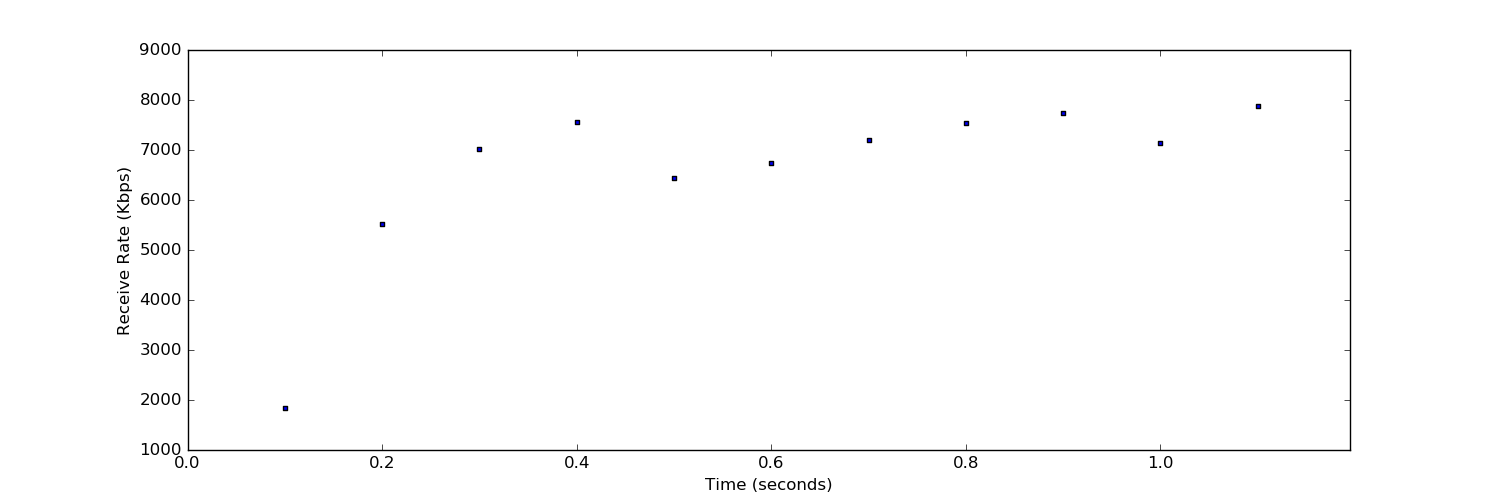
\includegraphics[width=\linewidth]{1f_rate.png}
\end{figure}

discuss competing RTT here

\end{enumerate}


\end{document}
